% DISCUSSION CONTENT


\section{Impact of this work}
In this work, we made scientific contributions to the field of computational biology applied to single-cell omics. More specifically, we developed approaches for performing trajectory inference and network inference analyses for single-cell omics, as well as approaches for assessing the performance of such methods in a quantitative way.

The contribution with the largest impact in the field is the large-scale comparison of 45 TI methods. Based on our results, we provided guidelines on how to perform a TI analysis and developed a toolkit for performing a inferring and interpreting trajectories using any of these methods. Since such guidelines were hitherto lacking, they are now commonly disseminated in manuscripts \cite{lafzi_tutorialguidelinesexperimental_2018, luecken_currentbestpractices_2019}, courses \cite{kiselev_analysissinglecell_2019, martens_analysissinglecell_2019}, and slides shown during keynote caffeine refuelling sessions \cite{hemberg_coffeebreakanalysis_2019}. These disseminations are having a significant impact in how TI analyses are being performed in academia and industry alike.

This dissertation commences with a rant on low self-assessment rates of method developers. As a result, we developed a simulator of \textit{in silico} single cells, that allow quantifying the accuracy the prediction of a tool, even if the real data required to perform this analysis does not exist yet. While the manuscript is not published yet, dyngen has already been used to evaluate trajectory inference \cite{saelens_comparisonsinglecelltrajectory_2019}, trajectory-based differential expression \cite{vandenberge_trajectorybaseddifferentialexpression_2019}, and network inference \cite{pratapa_benchmarkingalgorithmsgene_2019} methods. 


% has used dyno detomaso_functionalinterpretationsingle_2019

\section{Outlook}
The types of computational analyses presented in Section~\ref{sec:comptools} (Clustering, DE, DR, TI, NI) have all become routine methodologies for analysing and interpreting single-cell omics data. With projects like the Human Cell Atlas\cite{humancellatlasconsortium_humancellatlas_2018} soon to be churning out millions of single-cell profiles on a regular basis, research in high-throughput computational tools to analyse these data in an unsupervised approach becomes increasingly relevant. 

Here, we discuss several promising categories of computational methods (Figure~\ref{fig:scapplications_extended}) that are mostly in an exploratory stage but show promising results towards becoming another major computational workhorse in single-cell biology.

\begin{figure}[htb!]
	\centering
	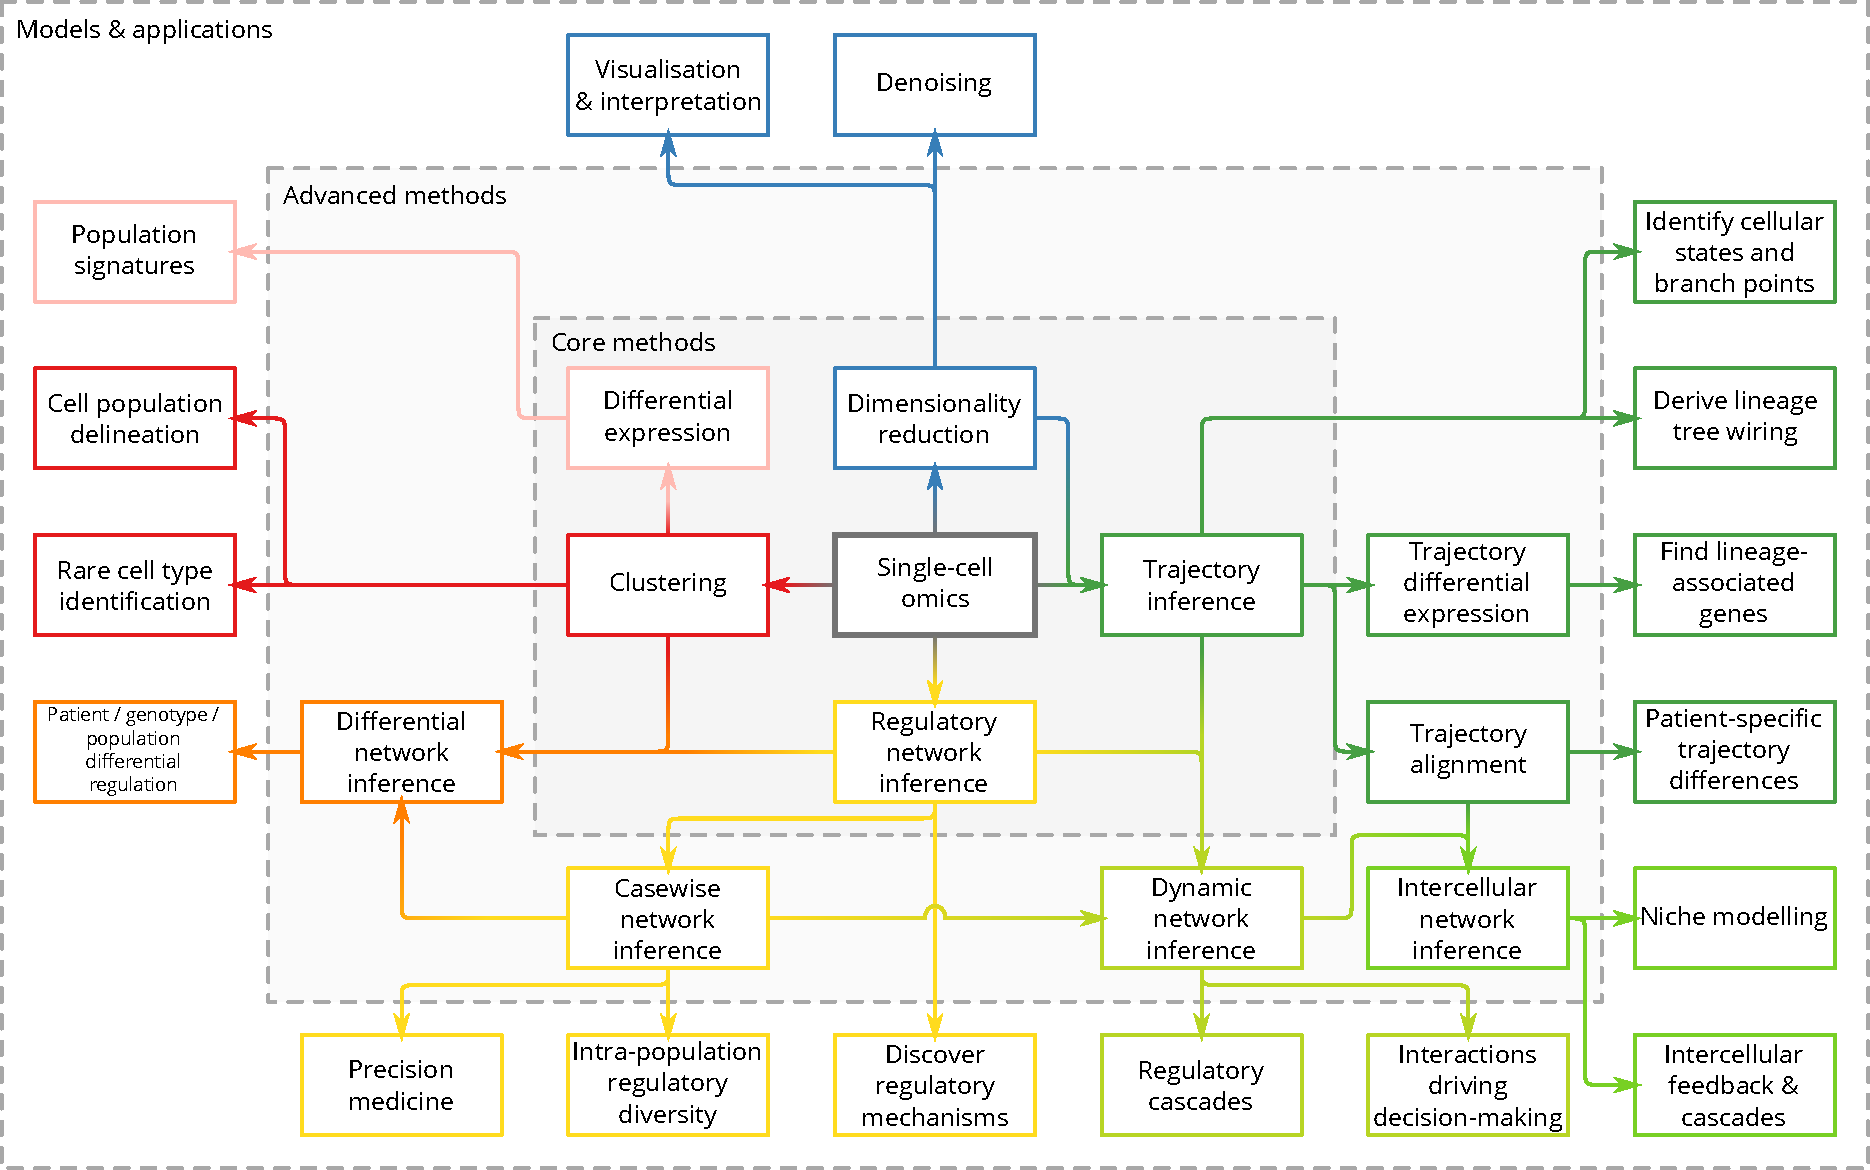
\includegraphics[width=\linewidth]{fig/singlecell_technologies_v8.pdf}
	\caption{Developments in computational methods for single-cell omics. Adapted from presentations by Wouter Saelens and myself.}
	\label{fig:scapplications_extended}
\end{figure}


\subsection{Trajectory differential expression}
Trajectory inference methods have made transformative changes in single-cell omics by allowing to study how cells change during a dynamic process of interest in a high-throughput and unsupervised approach. 
A crucial aspect in analysing and interpreting the resulting trajectories is the discovery of genes whose expression significantly shifts in a region of interest within the trajectory, called Trajectory Differential Expression (TDE).

Several trajectory inference methods offer TDE functionality as part of downstream analysis and interpretation of the outputted trajectories \cite{cannoodt_scorpiusimprovestrajectory_2016,qiu_reversedgraphembedding_2017,lonnberg_singlecellrnaseqcomputational_2017,wolf_pagagraphabstraction_2019}. However, current approaches typically cluster cells and perform differential expression analyses between the clusters, or are otherwise limited towards detecting differential expression of a gene along linearly ordered cells along one lineage path in the trajectory.

tradeSeq \cite{vandenberge_trajectorybaseddifferentialexpression_2019} is a generalised TDE method which can be used to discover different types of differential expression along a trajectory, which can be applied as a downstream analysis to trajectories inferred from any TI method. By including a comparative benchmark of TDE methods on real and synthetic data, Van den Berge et al. started a rational dialogue on TDE methodology.

\subsection{Trajectory alignment}
Trajectory alignment allows studying the differences between multiple trajectories that are mostly similar. For example, the cell developmental process of a patient could be compared to that of a healthy control to detect the transcriptomic differences of a particular lineage branch. 

Trajectory alignment has been used to compare gene expression kinetics resulting from different biological processes\cite{cacchiarelli_aligningsinglecelldevelopmental_2018}, to compare human, chimpanzee and macaque neuronal development\cite{kanton_organoidsinglecellgenomic_2019}, to find differences in gene regulation in the presence of certain growth factors\cite{mcfaline-figueroa_pooledsinglecellgenetic_2019}, and to compare human and mouse embryogenesis\cite{alpert_alignmentsinglecelltrajectories_2018}.

However, aligning trajectories becomes exponentially more difficult as the complexity of compared trajectories increases. For this reason, trajectory alignment remains a mostly unexplored territory within single-cell omics.

Dynamic Time Warping (DTW) \cite{giorgino_computingvisualizingdynamic_2009} is most commonly used to align linear trajectories. DTW is a technique originating in the field of speech recognition and aligns temporal sequences by creating a warping path between two sequences that indicates which sequence must be dilated or contracted to best match the other one.

Over time, as the affordability of single-cell omics technologies improves and the abundance of available datasets increases, we hypothesize that these methods will become highly relevant in comparing dynamic processes in samples from multiple donors.

\subsection{Variations on network inference}
Using a collection of transcriptomic profiles, network inference (NI) methods predict which genes are the regulators of a target gene. The output of an NI method is called a gene regulatory network in which each predicted interaction can be assigned a predicted strength or effect (activating or inhibitory).
However, cells are very molecularly heterogeneous, and only a fraction of all possible gene regulatory interactions is active at any point in time. Unfortunately, 'bulk' NI does not permit studying the diversity of regulatory activity within and between cell populations, and will thus suffer from similar drawbacks as bulk omics when compared to single-cell omics. Several adaptations of NI have been developed to address this problem, namely Differential NI, Dynamic NI, Casewise NI and Intercellular NI. 

\textbf{Differential NI} methods reconstruct one network per group of cells. The grouping can either be defined by prior knowledge, for example from gene expression, clustering, or by sorting the cells \textit{a priori}. 
The resulting networks can be investigate to detect differentially active (groups of) interactions between conditions (e.g. deregulated pathways between healthy and diseased), or (groups of) interactions that are highly active in between conditions (e.g. for investigating common pathways between different conditions). Differential NI methodology had already been developed for bulk omics \cite{ideker_differentialnetworkbiology_2012} to, for example, infer deregulated regulatory mechanisms in different subtypes of leukaemia \cite{gill_differentialnetworkanalysis_2014}.
Recently, similar methodology has been discussed in the context of single-cell omics as well \cite{chiu_scdnetcomputationaltool_2018}.

\textbf{Dynamic NI} methods exploit cell ordering information to improve the resulting regulatory network. Prior ordering information can be obtained experimentally (e.g. by performing lineage tracing or time-series experiments) or computationally (e.g. by performing trajectory inference or RNA velocity experiments). Unfortunately, most methods which are labelled as dynamic NI methods use time-series information to augment the inference of a static network. Ideally, dynamic NI methods would predict how the activity of interactions change along (pseudo-)time, as doing so would allow to detect regulatory cascades or interactions which act as the main drivers behind crucial dynamic processes.

In \textbf{casewise NI}, one regulatory network is predicted for every single-cell in the dataset. Doing so allows studying the heterogeneity (or homogeneity) between and within different cell populations. In essence, most analyses that can be run on single-cell omics (e.g. diffential expression) can also be applied on casewise regulatory networks (e.g. to predict differentially expressed interactions).
It is the most generalised form of NI of the variants discussed above, as a casewise regulatory network can be clustered to create a differential network, or trajectory inference can be applied to derive a dynamic regulatory network. Examples of casewise NI methods include SCENIC \cite{aibar_scenicsinglecellregulatory_2017}, SSN \cite{liu_personalizedcharacterizationdiseases_2016}, and LIONESS \cite{kuijjer_estimatingsamplespecificregulatory_2019}.

Instead of inferring gene regulatory mechanisms occurring within a cell, \textbf{intercellular NI} methods \cite{efremova_cellphonedbv2inferring_2019,browaeys_nichenetmodelingintercellular_2019} study communication between cells by predicting interactions between the ligands of one type of cells and the receptors of another group of cells. Such methods typically require much more prior data (e.g. which cells are communicating with which cells, what are the ligands and receptors), but allows studying how the cells react to their environment and investigate intercellular feedback mechanisms. 



\section{A life without Git, Travis CI, or tidyverse}
A significant portion of this work involved developing large software libraries, in a collaborative setting, over a time span of about four years. Since the results of our comparison of 45 TI methods required three years to develop, we were happily forced to develop a system where experiments could be rerun and results could be updated on-the-fly.

We summarised our experiences in the form of a set of guidelines for benchmarking computational tools (Chapter~\ref{chap:guidelines}). However, these guidelines do not touch upon many aspects of good software development practices that we learned to use in order to bring this thesis to a good end. In particular, I would like to highlight several  fundamental (open-source) projects without the likes of which our research would have been simply impossible to perform, namely Git, Travis CI, and the tidyverse.

\textbf{Git} \cite{torvalds_gitfastversion_2005} is a code-revision system that allows multiple users to collaborate on developing code and keep track of what changes were made by whom. 
Since Wouter Saelens and I were often working closely together on a specific part of our software, Git saved us a lot of time by merging together changes developed in parallel. Only in few cases did we need to intervene manually to merge our changes.
Additionally, Github.com allowed us not only to collaborate with each-other, but also correspond and collaborate with other software developers from many different research groups, using Github Issues to discuss problems with other researchers, and Github Pull Requests to contribute code to open-source projects. 

Together, we published over 20'000 code contributions (commits) across 50+ software packages \cite{cannoodt_developmentdynverse_2019}. Since many of these packages depend on one another, it is inevitable that changes made to one package would break another package. We wrote many, many unit tests (and still too few), and we let these tests automatically be executed on \textbf{Travis CI} \cite{traviscigmbh_traviscitest_2011}. This way, when we pushed breaking changes to Github, Travis CI would notify that our commit has resulted in one or more unit tests failing. While sometimes it is a hassle to set up, Travis CI has prevented us countless times from generating faulty results due to a faulty underlying function.

Software bugs can be introduced even by incredibly small, seemingly insignificant changes. The R programming language seems particularly susceptible towards getting trapped by its many pitfalls. However, there are many benefits of using R in bioinformatics research context, such as its extensive community of statisticians develop packages for the R ecosystem. The \textbf{tidyverse} packages \cite{wickham_welcometidyverse_2019}, developed by the RStudio team and many online contributors, completely transformed my experiences with R from tedious struggles to efficient everyday functional programming.

Honourable mentions are Linux, Fedora, \LaTeX, TeXstudio, (R)Markdown, Bash, Sed, Regular expressions, Rocket Chat, for making bioinformatics software development even more fun and enjoyable.

\clearpage
\section{References}
\printbibliography[heading=none]
